% 05.tex -- подключается к main.tex.
% Ответы для учителя: 3) 72; 60. 4) x = 228.
% 5) 50 сторон. 6) 75 м/мин.
% 7) 840 : 35 = 24; промежуточные числа: 70, 140, 140.
% Самостоятельная работа: 1) 24 апельсина; 2) 44, 45, 46.

\begingroup
\setlength{\emergencystretch}{2em}

{\large\bfseries
5. Деление на двузначное число\par}
\nobreak\vspace{0.4em}

\begin{enumerate}[
    label={\fbox{\bfseries\arabic*}},
    leftmargin=*,
    labelsep=0.5em,
    itemsep=0.6em,
    topsep=0.3em,
    parsep=0pt
]

\item Чёрный ящик. Нужно угадать делитель, если известен остаток от деления.

\item \textbf{Деление на двузначное число} на примере $936:24$;  $12285:21$.

\item Выполните деление в столбик:
\[
\text{а)}\;1728:24; \qquad \text{б)}\;3480:58.
\]

\item Решите уравнение:
\[
23\cdot(x-156):24+18=87.
\]

\item Периметр многоугольника равен $1800$~дм,
а длина одной стороны --- $360$~см. Все стороны
многоугольника равны. Сколько у него сторон?

\item Никита вышел из дома в 8:12 и побежал в школу
со скоростью $150$~м/мин. В школу он зашёл ровно
со звонком, в 8:30. Обратно он шёл той же дорогой
вместе с другом Сашей и потратил на весь обратный путь
$36$~минут. С какой скоростью Никита шёл обратно?

\item Восстановите пропущенные цифры:

\par\nobreak\vspace{0.15em}\nobreak
\centerline{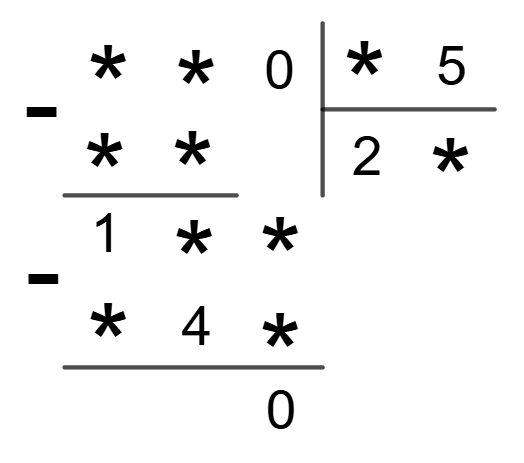
\includegraphics[height=2.8cm]{images/05-division-rebus.png}}

\end{enumerate}

\newpage

{\large\bfseries Самостоятельная работа\par}
\nobreak\vspace{0.5em}

\begin{enumerate}[
    label={\fbox{\bfseries\arabic*}},
    leftmargin=*,
    labelsep=0.5em,
    itemsep=1em,
    topsep=0.4em,
    parsep=0pt
]

\item Из $15$ апельсинов получается $10$ стаканов сока.
Сколько надо взять апельсинов, чтобы получилось
$16$ стаканов сока?

\vspace{1.7cm}

\item На доске было записано три последовательных числа.
Когда стёрли одно, то сумма оставшихся чисел стала равна $90$.
Какие числа были записаны на доске?

\vspace{1.7cm}

\item Серёжа разрезал квадрат на две части и сложил
из них такую фигуру. Определите, на какие части был
разрезан квадрат, и закрасьте каждую из них своим цветом.

\begin{center}
\begin{tikzpicture}[x=0.65cm,y=0.65cm]
    % Рамка из 16 клеток, как на исходном скриншоте.
    \draw[line width=0.7pt] (0,0) rectangle (7,3);
    \draw[line width=0.7pt] (1,1) rectangle (6,2);
    \draw[line width=0.4pt] (0,1) -- (7,1);
    \draw[line width=0.4pt] (0,2) -- (7,2);
    \foreach \x in {1,...,6} {
        \draw[line width=0.4pt] (\x,0) -- (\x,1);
        \draw[line width=0.4pt] (\x,2) -- (\x,3);
    }
    \draw[line width=0.4pt] (1,1) -- (1,2);
    \draw[line width=0.4pt] (6,1) -- (6,2);
\end{tikzpicture}
\end{center}

\end{enumerate}
\endgroup
